\documentclass[letterpaper,12pt]{article}
\usepackage[letterpaper]{geometry}
\usepackage[english]{babel}
\usepackage{empheq}
\usepackage{graphicx}
\usepackage{epstopdf}

\special{papersize=8.5in,11in}

\begin{document}

\begin{titlepage}
\newcommand{\HRule}{\rule{\linewidth}{0.5mm}} % Defines a new command for the horizontal lines, change thickness here

\center % Center everything on the page
%----------------------------------------------------------------------------------------
%	HEADING SECTIONS
%----------------------------------------------------------------------------------------

\textsc{\LARGE University of Hong Kong}\\[1.5cm] % Name of your university/college
\vspace{2.5cm}
\textsc{\Large COMP 3270 Artificial Intelligence }\\[0.5cm] % Major heading such as course name
\textsc{\large Fall term 2017}\\[0.5cm] % Minor heading such as course title

%----------------------------------------------------------------------------------------
%	TITLE SECTION
%----------------------------------------------------------------------------------------

\HRule \\[0.4cm]
{ \LARGE \bfseries Report of Mini Project - Othello}\\[0.4cm] % Title of your document
\HRule \\[1.5cm]
 
%----------------------------------------------------------------------------------------
%	AUTHOR SECTION
%----------------------------------------------------------------------------------------

\begin{minipage}{0.8\textwidth}
\begin{center} \large
\vspace{0.5cm}

Qiu Haoran \\ \vspace{0.3cm}\textsc{UID: 3035234478}\\
\vspace{2cm}
\end{center}
\end{minipage}

%----------------------------------------------------------------------------------------
%	DATE SECTION
%----------------------------------------------------------------------------------------

{\large 28/November/2017}\\[3cm] % Date - could also use \today

%----------------------------------------------------------------------------------------
%	LOGO SECTION
%----------------------------------------------------------------------------------------

%\includegraphics{Logo}\\[1cm] % Include a department/university logo - this will require the graphicx package
 
%----------------------------------------------------------------------------------------

\vfill % Fill the rest of the page with whitespace
\end{titlepage} 

\begin{abstract}
Othello, also named Reversi, is a strategy board game between the player and an artificial intelligent opponent. This report describes in detail about the methodology, such as the architecture, search engine, $\alpha$-$\beta$ pruning, heuristics applied, and the evaluation function in use. Some other detail about the program like the number of steps the AI looks ahead, and the database in use.
\end{abstract}

\section{Game Modeling}
\textbf{Initial State}: Initial game board is an 8 by 8 board with four disks placed in the center like the figure bellow.
\begin{figure}[!htb]
\centering
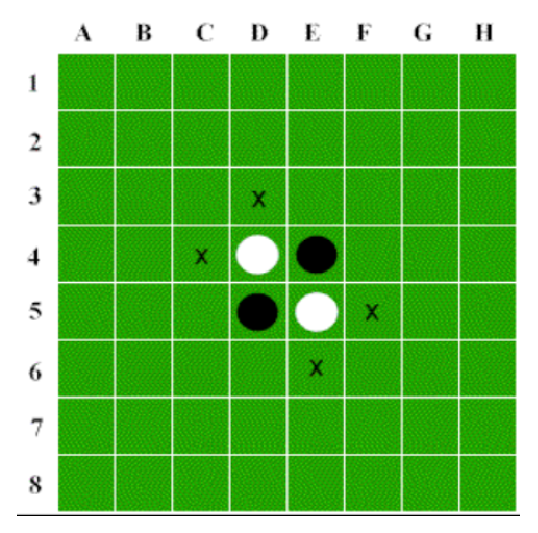
\includegraphics[scale=.6]{initial.eps}
\caption{Initial Board \& Possible Move}
\label{fig:digraph}
\end{figure}
\\
\noindent
\textbf{Players}: The game is a two-player game. One is the user, and the other is the computer. The player places black disks while the computer places white ones. The user is the first to play and then two players place disks alternatively. If one of the two players does not have any legal moves, then this player pass his turn to the other player.
\\\\
\textbf{Actions}: Each player should place the disk to a position where the unplaced one can surround disk(s) with another same-color disk horizontally, vertically, or diagonally. In figure 1, the legal movements for the black are marked by cross signs.
\\\\
\textbf{Result(state,move)}: The transition model, which defines the result of a move.
\\\\
\textbf{Terminal Test}: The game is over when there's no legal move for both two players or the board is full.
\\\\
\textbf{Utility(state, player)}: A utility function defining a numerical value for the player at a particular state.
\\\\
The initial state, actions, and result(transition model) define the game tree for Othello - a tree where the nodes are game states and the edges are moves. It's also called a search tree is it's superimposed on the full game tree, and examines enough nodes to allow a player to determine what move to make.


\section{Methodology}
\subsection{Search Engine}
\subsection{$\alpha$-$\beta$ Pruning}
\subsection{Heuristics Applied}
\subsection{Evaluation Function}


\section{Program Architecture}


\section{Others}


\begin{thebibliography}{}
\bibitem{}
Reversi, Wikipedia, September 2017, https://en.wikipedia.org/wiki/Reversi
\end{thebibliography}
\end{document}